\documentclass{article}
\usepackage[protrusion=true]{microtype}
\usepackage[sfdefault]{FiraSans}
\usepackage[T1]{fontenc}
\usepackage[utf8]{inputenc}
\usepackage{algorithm}
\usepackage{algorithmic}
\usepackage{amsfonts}
\usepackage{amsmath}
\usepackage{amssymb}
\usepackage[style=apa]{biblatex}
\usepackage{booktabs}
\usepackage{breqn}
\usepackage{enumitem}
\usepackage{float}
\usepackage{geometry}
\usepackage{graphicx}
\usepackage{hyperref}
\usepackage{lipsum}
\usepackage{listings}
\usepackage{longtable}
\usepackage{multirow}
\usepackage{pdfpages}
\usepackage{pgfgantt}
\usepackage{setspace}
\usepackage{subcaption}
\usepackage{tabularx}
\usepackage{tikz}
\usepackage{xcolor}

% Set bibliography style to APA
\DeclareLanguageMapping{english}{english-apa}

% Import bibliography file
\addbibresource{references.bib}

% Page layout
\geometry{letterpaper, left=1in, right=1in, top=1in, bottom=1in}

% Color scheme
\definecolor{primary}{RGB}{0,120,215}
\definecolor{secondary}{RGB}{255,87,34}
\definecolor{background}{RGB}{245,245,245}
\definecolor{blue}{RGB}{0,62,126}

% Page color (optional, can be removed if not needed)
\pagecolor{background}

% Hyperlink colors
\hypersetup{
    colorlinks=true,
    linkcolor=primary,
    filecolor=secondary,
    urlcolor=primary,
    citecolor=black
}

% Bibliography hyperlink colors
\AtBeginBibliography{\hypersetup{urlcolor=black}}

% Line spacing
\setstretch{1.15}

% Indent each reference by 0.5in on the second line
\setlength{\bibhang}{0.5in}

% Put space between bibliography items
\setlength\bibitemsep{1.5\itemsep}

% No paragraph indentation
\setlength{\parindent}{0pt}

\begin{document}

\newcommand{\mytitlepage}[2]{
    \thispagestyle{empty}

    \begin{tikzpicture}[remember picture, overlay]
        % Place the background image at the bottom-left corner and extend it over the entire page
        \node [anchor=south west, inner sep=0pt] at (current page.south west) {
            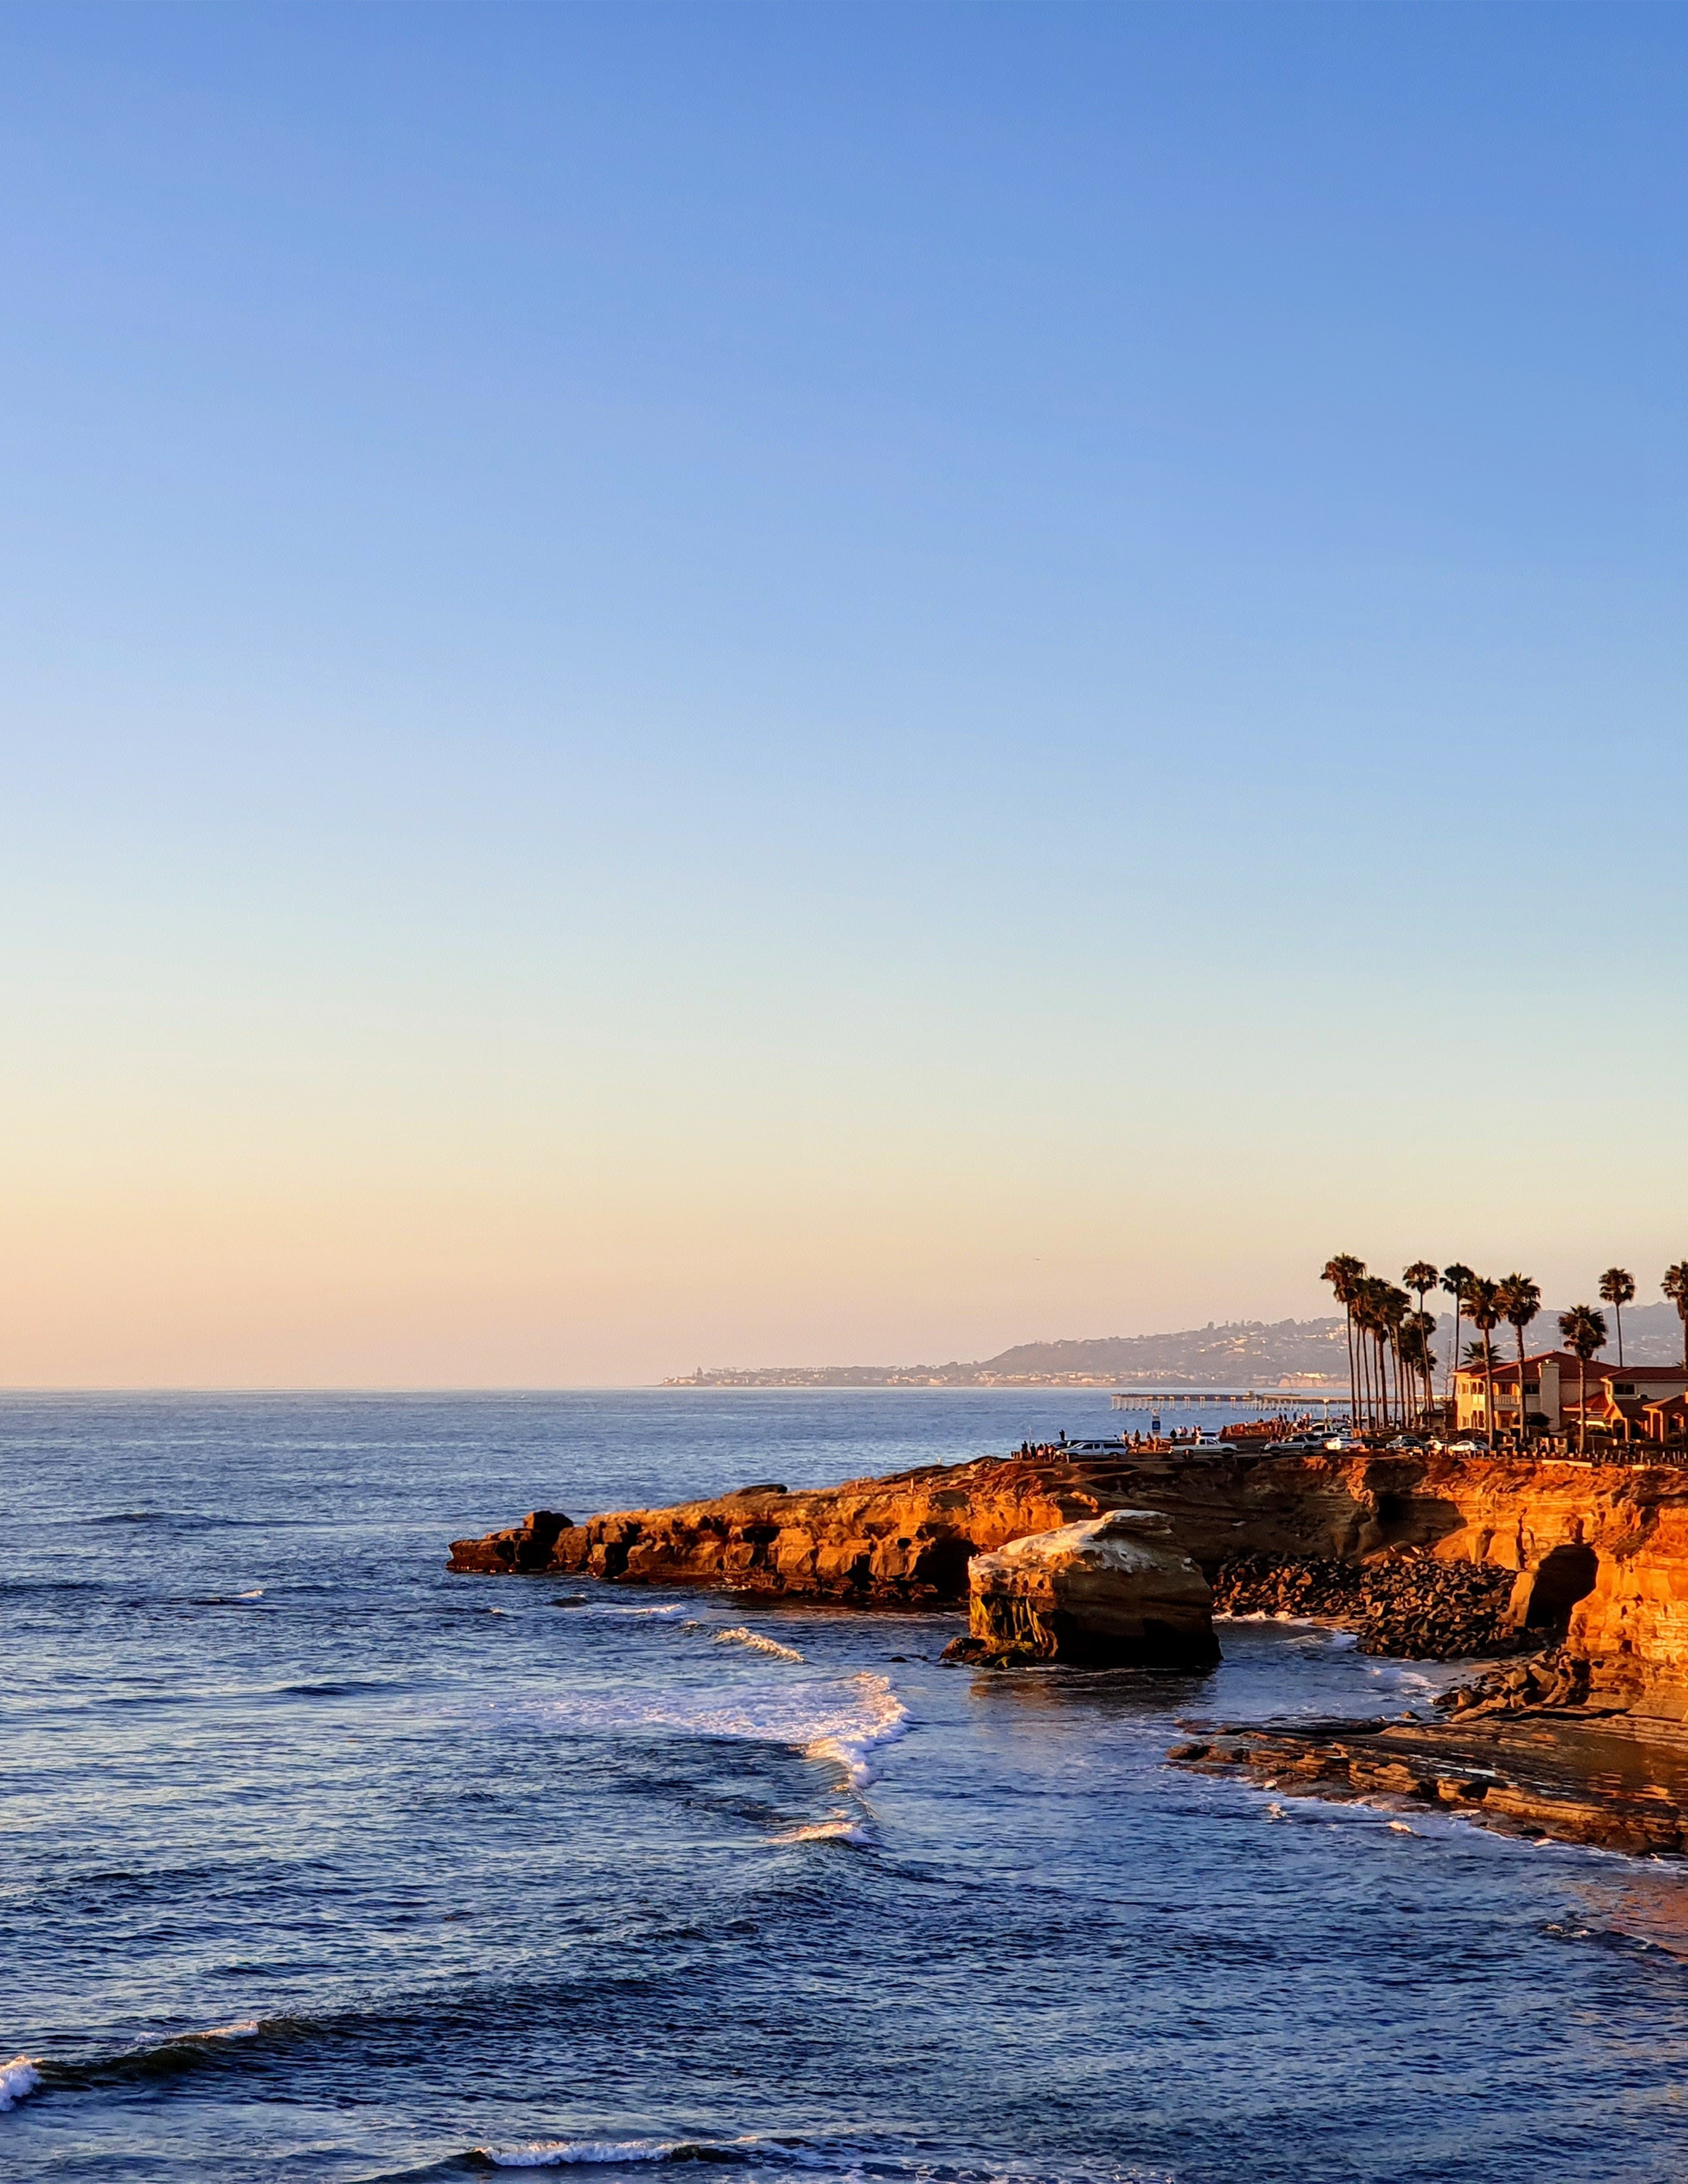
\includegraphics[width=\paperwidth,height=\paperheight]{images/background.png}
        };
        {
            \node [
                anchor=center,
                inner sep=1.25cm,
                rectangle,
                fill=blue!70!white,
                fill opacity=0,
                text opacity=1,
                minimum height=0.2\paperheight,
                minimum width=\paperwidth,
                text width=0.8\paperwidth,
                font=\fontfamily{pnc}\selectfont
            ] at (current page.center) {#2};
        }
        \node [anchor=south east, outer sep=3pt] at (current page.south east) {
            \includegraphics[width=0.33\paperwidth]{images/logo.png}
        };
    \end{tikzpicture}

    \newpage
}

{
    \mytitlepage{}{
        \centering
        \fontfamily{phv}

        \vspace{-200pt} % move title up

        {
            \Huge
            \bfseries
            Diabetic Readmission Risk Prediction
            \par
        }

        \vspace{8pt}

        {
            \Large
            \bfseries
            Design Document
            \par
        }

        \vspace{24pt}

        {
            \begin{center}
                \begin{tabular*}{\textwidth}{@{\extracolsep{\fill}}c c c}
                    {\LARGE Jonathan Agustin} & {\LARGE Zack Robertson} & {\LARGE Lisa Vo}
                \end{tabular*}
            \end{center}
        }
    }
}

\newpage
\tableofcontents
\newpage

\pagenumbering{arabic}

\section{Introduction}

Hospital readmissions, particularly within 30 days of discharge, represent a significant challenge to healthcare systems worldwide, leading to increased costs and potentially adverse patient outcomes. Diabetic patients are especially vulnerable to readmission due to the chronic and complex nature of diabetes management. This document outlines the design of a machine learning (ML) system aimed at predicting 30-day hospital readmissions among diabetic patients. By leveraging historical patient data and advanced analytical techniques, the system seeks to identify high-risk individuals, enabling proactive interventions and contributing to improved healthcare efficiency and patient well-being.

\section{Problem Statement}

The rising rate of hospital readmissions among diabetic patients presents a multifaceted problem for healthcare providers. It strains resources, increases healthcare expenditures, and can negatively impact patient health and quality of life. The complexity of diabetes management, potential complications, and the need for strict adherence to treatment regimens contribute to the elevated readmission risk for this population.

This project addresses the challenge of accurately predicting 30-day hospital readmissions among diabetic patients. By developing a robust and scalable machine learning system, we aim to analyze a wide range of patient attributes—including demographics, medical history, treatment patterns, and hospital procedures—to identify individuals at high risk of readmission. This predictive capability will empower clinicians to implement targeted interventions, potentially reducing readmission rates and improving overall patient care.

\section{Impact Measurement}

To assess the effectiveness of the ML system, we will employ a comprehensive set of metrics and analyses. These measures are designed to evaluate not only the technical performance of the model but also its real-world impact on healthcare delivery.

\subsection{Model Performance Metrics}

The predictive accuracy and reliability of the model are critical for its adoption in clinical settings. We will utilize the following standard classification metrics:

\begin{itemize}[leftmargin=*]
    \item \textbf{Accuracy}: Measures the proportion of correct predictions out of all predictions.
    \item \textbf{Precision}: Assesses the model's ability to correctly identify true positive cases among all positive predictions.
    \item \textbf{Recall (Sensitivity)}: Evaluates the model's capacity to identify all actual positive cases.
    \item \textbf{F1-Score}: Represents the harmonic mean of precision and recall, providing a balance between the two.
    \item \textbf{ROC-AUC Score}: Quantifies the model's ability to distinguish between classes by plotting the true positive rate against the false positive rate.
\end{itemize}

These metrics will be calculated on a held-out test dataset to provide an unbiased evaluation of the model's performance.

\subsection{Reduction in Readmission Rates}

A key goal of deploying the ML system is to achieve a measurable reduction in readmission rates among diabetic patients. We plan to:

\begin{itemize}[leftmargin=*]
    \item \textbf{Establish a Baseline}: Determine the current readmission rate prior to implementing the ML system.
    \item \textbf{Post-Implementation Monitoring}: Track readmission rates following deployment to assess changes.
    \item \textbf{Target Reduction}: Aim for at least a 10\% decrease in 30-day readmission rates, indicating a significant positive impact.
\end{itemize}

Comparing these rates before and after implementation will help us assess the practical benefits of the system in a real-world healthcare environment.

\subsection{Cost Savings Analysis}

Reducing readmissions can result in substantial cost savings for healthcare institutions. We will analyze:

\begin{itemize}[leftmargin=*]
    \item \textbf{Direct Cost Savings}: Calculate the reduction in expenses associated with fewer hospital stays, treatments, and procedures for readmitted patients.
    \item \textbf{Indirect Cost Savings}: Consider savings from improved resource allocation, such as reduced burden on hospital staff and facilities.
    \item \textbf{Return on Investment (ROI)}: Evaluate the financial benefits in relation to the costs incurred in developing and deploying the ML system.
\end{itemize}

This analysis will provide insights into the economic value of the system for healthcare providers.

\subsection{Resource Optimization}

Efficient utilization of healthcare resources is essential for enhancing patient care while controlling costs. We will examine:

\begin{itemize}[leftmargin=*]
    \item \textbf{Bed Occupancy Rates}: Assess changes in bed availability and whether reduced readmissions lead to better management of hospital capacity.
    \item \textbf{Staff Workload}: Evaluate the impact on healthcare provider workloads, aiming for a more balanced distribution of patient care duties.
    \item \textbf{Preventive Care Allocation}: Observe whether resources can be reallocated towards preventive measures and patient education due to reduced readmissions.
\end{itemize}

By monitoring these indicators, we can validate the system's contribution to overall healthcare efficiency and patient care quality.

\section{Security, Bias, and Ethical Considerations}

In developing an ML system for healthcare, it is imperative to address security, bias, and ethical concerns comprehensively. Patient data is sensitive and subject to strict regulations, and the ML models must be fair and transparent in their predictions.

\subsection{Security Checklist}

\begin{itemize}[leftmargin=*]
    \item \textbf{Data Privacy Compliance}: Compliance with the Health Insurance Portability and Accountability Act (HIPAA) is mandatory. We will implement strict data governance policies to ensure patient confidentiality. Data de-identification techniques will remove personally identifiable information (PII), and any data sharing will adhere to consent agreements and legal requirements.
    \item \textbf{Secure Data Storage}: All data will be stored in encrypted Amazon S3 buckets using server-side encryption (SSE-S3). Access will be controlled through AWS Identity and Access Management (IAM) roles and policies, restricting permissions to authorized personnel only. Regular backups and recovery tests will prevent data loss.
    \item \textbf{Data Transmission Security}: We will enforce HTTPS protocols for all data transmission between services, utilizing SSL/TLS encryption to protect data in transit against interception and unauthorized access.
    \item \textbf{Access Control}: Role-Based Access Control (RBAC) will define user permissions based on specific roles and responsibilities. Regular audits of access logs will be conducted to detect and respond to any unauthorized activities.
    \item \textbf{Incident Response Plan}: A comprehensive incident response strategy will be developed, outlining procedures for incident detection, containment, eradication, recovery, and follow-up. Roles and responsibilities will be clearly defined to ensure an effective response to any security incidents.
\end{itemize}

\subsection{Bias and Ethical Concerns}

\begin{itemize}[leftmargin=*]
    \item \textbf{Bias Identification and Mitigation}: We recognize the potential for biases related to age, gender, race, or socioeconomic status. Regular audits will be performed to detect such biases using techniques like Disparate Impact Analysis. If biases are identified, we will adjust training data and model parameters to ensure equitable treatment across all patient groups.
    \item \textbf{Model Explainability and Transparency}: To foster trust and facilitate clinical adoption, we will employ interpretable models or integrate explainability tools such as SHAP (SHapley Additive exPlanations). This approach provides clinicians with clear insights into the factors influencing each prediction.
    \item \textbf{Informed Consent and Data Usage}: Patient consent forms will include authorization for data usage in predictive modeling. Transparency about data collection methods, storage practices, and purposes will be maintained to build trust with patients and stakeholders.
    \item \textbf{Compliance with Ethical Guidelines}: The project will align with ethical standards set by professional bodies like the American Medical Association (AMA). Training will be provided to staff on data ethics, privacy, and responsible AI practices to cultivate an ethical culture.
\end{itemize}

By proactively addressing these considerations, we aim to build a system that is not only effective but also trustworthy and respectful of patient rights.

\section{Solution Overview}

Our proposed solution integrates robust data handling, advanced modeling techniques, seamless deployment strategies, and continuous monitoring processes. Each component is designed to contribute to an effective and reliable ML system for predicting hospital readmissions.

\subsection{System Architecture}

The overall architecture of the proposed ML system is designed to facilitate seamless data flow, robust model training, and efficient deployment. The system comprises multiple components, each responsible for specific tasks, integrated to function cohesively.

\subsubsection{System Architecture Diagram}

\begin{figure}[H]
    \centering
    % Include the architecture diagram here
    \begin{tikzpicture}[node distance=1.8cm, auto, scale=0.8, transform shape]
        \node [draw, rectangle, text centered, minimum width=2cm] (DataSources) {Data Sources};
        \node [draw, rectangle, text centered, below of=DataSources] (DataIngestion) {Data Ingestion};
        \node [draw, rectangle, text centered, below of=DataIngestion] (DataStorage) {Data Storage};
        \node [draw, rectangle, text centered, below of=DataStorage] (DataEngineering) {Data Engineering};
        \node [draw, rectangle, text centered, below of=DataEngineering] (FeatureEngineering) {Feature Engineering};
        \node [draw, rectangle, text centered, below of=FeatureEngineering] (ModelTraining) {Model Training};
        \node [draw, rectangle, text centered, right=2.5cm of ModelTraining] (ModelDeployment) {Model Deployment};
        \node [draw, rectangle, text centered, right=2.5cm of ModelDeployment] (APIEndpoint) {API Endpoint};
        \node [draw, rectangle, text centered, above of=APIEndpoint] (ClinicalApplication) {Clinical Application};
        \node [draw, rectangle, text centered, above of=ClinicalApplication] (HealthcareProviders) {Healthcare Providers};

        \draw [->] (DataSources) -- (DataIngestion);
        \draw [->] (DataIngestion) -- (DataStorage);
        \draw [->] (DataStorage) -- (DataEngineering);
        \draw [->] (DataEngineering) -- (FeatureEngineering);
        \draw [->] (FeatureEngineering) -- (ModelTraining);
        \draw [->] (ModelTraining) -- (ModelDeployment);
        \draw [->] (ModelDeployment) -- (APIEndpoint);
        \draw [->] (APIEndpoint) -- (ClinicalApplication);
        \draw [->] (ClinicalApplication) -- (HealthcareProviders);
        \draw [->, dashed] (HealthcareProviders.north) to[bend left=45] node[midway, right]{Feedback Loop} (DataSources.east);

    \end{tikzpicture}
    \caption{System Architecture Diagram}
    \label{fig:system_architecture}
\end{figure}

\textit{Figure \ref{fig:system_architecture}: System Overview Diagram illustrating the flow from data sources through model deployment to clinical application and feedback integration.}

\subsection{Data Sources}

We utilize the \textbf{Diabetes 130-US hospitals for years 1999-2008 Data Set} from the UCI Machine Learning Repository, accessed via the Hugging Face Datasets library under the identifier \texttt{aai540-group3/diabetes-readmission}.

\subsubsection{Dataset Characteristics}

\begin{itemize}[leftmargin=*]
    \item \textbf{Size}: The dataset contains 101,766 patient records, providing a substantial sample for model training and evaluation.
    \item \textbf{Features}: It includes 55 attributes encompassing demographics (age, gender, ethnicity), medical history (diagnoses, comorbidities), laboratory results, medications, and hospitalization details (length of stay, number of procedures).
    \item \textbf{Target Variable}: The \texttt{readmitted} indicator (0 or 1) signifies whether a patient was readmitted within 30 days of discharge.
\end{itemize}

\begin{table}[H]
\centering
\caption{Summary of Dataset Features}
\label{tab:dataset_features}
\begin{tabular}{p{3cm} p{10cm}}
\toprule
\textbf{Feature Type} & \textbf{Description} \\
\midrule
Demographics & Age, Gender, Ethnicity \\
Medical History & Diagnoses (primary and secondary), Comorbidities \\
Lab Results & Number of lab procedures, lab test results \\
Medications & Number of medications, types of medications administered \\
Hospitalization Details & Length of stay, number of inpatient visits, number of procedures \\
Other & Discharge disposition, admission type, payer code \\
\bottomrule
\end{tabular}
\end{table}

\textit{Table \ref{tab:dataset_features}: Summary of the types of features included in the dataset.}

\subsubsection{Versioning}

\begin{itemize}[leftmargin=*]
    \item \textbf{Consistency}: The dataset is versioned (\texttt{v1.0}) to ensure consistency and reproducibility across different experiments and development stages.
    \item \textbf{Storage}: Raw data is stored in a structured format within the repository (\texttt{data/raw/data.csv}), enabling version control through tools like Git and DVC (Data Version Control).
\end{itemize}

\subsection{Data Engineering}

Effective data engineering is crucial for preparing the dataset for modeling. Our process entails data ingestion, cleaning, and splitting.

\subsubsection{Ingestion}

Using the custom script \texttt{ingestion.py}, we perform the following steps:

\begin{itemize}[leftmargin=*]
    \item \textbf{Data Loading}: Employ the Hugging Face Datasets API to reliably fetch the dataset.
    \item \textbf{Data Export}: Save the dataset as a CSV file in the \texttt{data/raw} directory, facilitating version control and transparency.
    \item \textbf{Logging}: Implement logging mechanisms to document the ingestion process, ensuring traceability and facilitating debugging if anomalies arise.
\end{itemize}

\subsubsection{Cleaning}

The \texttt{cleaning.py} script addresses data quality issues to enhance model performance:

\begin{itemize}[leftmargin=*]
    \item \textbf{Duplicate Removal}: Identified and removed 1,437 duplicate entries to prevent data redundancy and bias.
    \item \textbf{Missing Values Handling}:
        \begin{itemize}[leftmargin=*]
            \item \textbf{Numerical Variables}: Imputed missing values using the median, reducing the impact of outliers and skewed distributions.
            \item \textbf{Categorical Variables}: Filled missing values with the mode (most frequent value), maintaining category integrity.
        \end{itemize}
    \item \textbf{Data Type Consistency}:
        \begin{itemize}[leftmargin=*]
            \item Converted numerical features to \texttt{float32} for computational efficiency.
            \item Transformed binary categorical features into boolean types for clarity and proper handling in modeling.
        \end{itemize}
    \item \textbf{Feature Reduction}:
        \begin{itemize}[leftmargin=*]
            \item Removed features with more than 50\% missing data, such as \texttt{weight} and \texttt{payer\_code}, to avoid introducing bias or noise.
            \item Eliminated irrelevant identifiers (e.g., patient IDs) to prevent data leakage and protect privacy.
        \end{itemize}
    \item \textbf{Normalization and Standardization}: Applied where appropriate to ensure that features are on comparable scales, which is beneficial for certain algorithms.
\end{itemize}

\subsubsection{Splitting}

The \texttt{splitting.py} script divides the dataset into training and testing sets:

\begin{itemize}[leftmargin=*]
    \item \textbf{Training Set}: Consists of 80\% of the data, used for model training.
    \item \textbf{Testing Set}: Comprises 20\% of the data, reserved for evaluating model performance.
    \item \textbf{Stratification}: Ensured that the distribution of the target variable (\texttt{readmitted}) is consistent across both sets, maintaining the representativeness of the sample.
    \item \textbf{Reproducibility}: Used a fixed \texttt{random\_state=42} to enable consistent results in subsequent runs, facilitating collaboration and comparison.
\end{itemize}

\begin{figure}[H]
    \centering
    % Data engineering flowchart
    \begin{tikzpicture}[node distance=1.8cm, auto, scale=0.8, transform shape]
        \node [draw, rectangle, text centered] (Ingestion) {Data Ingestion};
        \node [draw, rectangle, text centered, below of=Ingestion] (Cleaning) {Data Cleaning};
        \node [draw, rectangle, text centered, below of=Cleaning] (FeatureEngineering) {Feature Engineering};
        \node [draw, rectangle, text centered, below of=FeatureEngineering] (Splitting) {Data Splitting};
        \draw [->] (Ingestion) -- (Cleaning);
        \draw [->] (Cleaning) -- (FeatureEngineering);
        \draw [->] (FeatureEngineering) -- (Splitting);
    \end{tikzpicture}
    \caption{Data Engineering Pipeline}
    \label{fig:data_engineering_pipeline}
\end{figure}

\textit{Figure \ref{fig:data_engineering_pipeline}: Data processing pipeline from ingestion to data splitting.}

\subsection{Feature Engineering}

Effective feature engineering can significantly enhance model performance by creating new variables that capture underlying relationships in the data.

\subsubsection{New Feature Creation}

Using \texttt{build\_features.py}, we engineered several new features:

\begin{table}[H]
\centering
\caption{Engineered Features}
\label{tab:engineered_features}
\begin{tabular}{p{4cm} p{10cm}}
\toprule
\textbf{Feature Name} & \textbf{Description} \\
\midrule
\texttt{total\_procedures} & Sum of \texttt{num\_lab\_procedures} and \texttt{num\_procedures}; represents the overall procedural burden. \\
\texttt{total\_visits} & Sum of \texttt{number\_outpatient}, \texttt{number\_emergency}, and \texttt{number\_inpatient}; reflects the frequency of healthcare interactions. \\
\texttt{avg\_procedures\_per\_visit} & \texttt{total\_procedures} divided by \texttt{total\_visits}; captures procedural intensity per visit. \\
\texttt{lab\_procedure\_ratio} & \texttt{num\_lab\_procedures} divided by \texttt{total\_procedures}; indicates the focus on diagnostic procedures. \\
\texttt{medication\_intensity} & \texttt{num\_medications} divided by \texttt{time\_in\_hospital}; captures the rate of medication administration. \\
\bottomrule
\end{tabular}
\end{table}

\textit{Table \ref{tab:engineered_features}: New features created during feature engineering.}

\subsubsection{Polynomial Features}

To capture non-linear relationships, we introduced polynomial features:

\begin{itemize}[leftmargin=*]
    \item \textbf{Implementation}: Used Scikit-learn's \texttt{PolynomialFeatures} with a degree of 2.
    \item \textbf{Application}: Applied to selected numerical features based on their correlation with the target variable.
    \item \textbf{Advantages}: Allows the model to learn complex patterns that linear features might not capture.
    \item \textbf{Considerations}: Monitored for potential issues such as multicollinearity and overfitting; performed feature selection post-generation to retain only features contributing positively to model performance.
\end{itemize}

\subsection{Model Training and Evaluation}

The modeling phase involved training two distinct models: Logistic Regression and AutoGluon's \texttt{TabularPredictor}. Both models were evaluated to determine their effectiveness.

\subsubsection{Models Implemented}

\paragraph{Logistic Regression}

\begin{itemize}[leftmargin=*]
    \item \textbf{Algorithm}: Utilized Scikit-learn's \texttt{LogisticRegression}, known for its simplicity and interpretability.
    \item \textbf{Hyperparameters}:
        \begin{itemize}[leftmargin=*]
            \item \textbf{Penalty}: L2 regularization to prevent overfitting.
            \item \textbf{Solver}: 'lbfgs', suitable for smaller datasets and supports L2 regularization.
            \item \textbf{Max Iterations}: Set to 1000 to ensure convergence, especially important given the complex feature set.
            \item \textbf{Random State}: Set to 42 for reproducibility.
        \end{itemize}
    \item \textbf{Preprocessing Steps}:
        \begin{itemize}[leftmargin=*]
            \item \textbf{Scaling}: Applied \texttt{StandardScaler} to standardize numerical features.
            \item \textbf{Imputation}: Used \texttt{SimpleImputer} to handle missing values.
            \item \textbf{Encoding}: Employed one-hot encoding for categorical variables.
        \end{itemize}
    \item \textbf{Training Process}:
        \begin{itemize}[leftmargin=*]
            \item Loaded preprocessed training data from \texttt{data/processed/logistic\_regression/train\_preprocessed.csv}.
            \item Trained the model and saved it as \texttt{models/logistic\_regression/model.pkl}.
        \end{itemize}
\end{itemize}

\paragraph{AutoGluon TabularPredictor}

\begin{itemize}[leftmargin=*]
    \item \textbf{Algorithm}: Leveraged AutoGluon's automated machine learning capabilities to systematically explore various models and hyperparameters.
    \item \textbf{Configuration}:
        \begin{itemize}[leftmargin=*]
            \item \textbf{Presets}: Set to 'best\_quality' to prioritize predictive performance.
            \item \textbf{Time Limit}: Restricted to 3600 seconds to balance computational resources and exploration depth.
            \item \textbf{Hyperparameters}: Customized settings for Gradient Boosting Machines (GBM) with \texttt{num\_boost\_round} set to 100.
            \item \textbf{Verbosity}: Level 2 to provide detailed logs during training.
        \end{itemize}
    \item \textbf{Automated Processing}:
        \begin{itemize}[leftmargin=*]
            \item AutoGluon handles missing values, categorical encoding, and feature scaling internally.
        \end{itemize}
    \item \textbf{Training Process}:
        \begin{itemize}[leftmargin=*]
            \item Used the raw training data (\texttt{data/processed/train.csv}).
            \item Trained models are stored under \texttt{models/autogluon/}.
        \end{itemize}
\end{itemize}

\subsubsection{Evaluation Metrics and Results}

Both models were evaluated on the test set, yielding the following results:

\begin{table}[H]
\centering
\caption{Model Performance Metrics}
\label{tab:model_performance}
\begin{tabular}{lcc}
\toprule
\textbf{Metric} & \textbf{Logistic Regression} & \textbf{AutoGluon} \\
\midrule
Accuracy & 46.01\% & 63.30\% \\
Precision & 69.49\% & 63.18\% \\
Recall & 46.01\% & 63.30\% \\
F1-Score & 46.01\% & 63.30\% \\
ROC-AUC & 64.65\% & 68.09\% \\
\bottomrule
\end{tabular}
\end{table}

\textit{Table \ref{tab:model_performance}: Comparison of model performance metrics.}

\paragraph{Analysis}

\begin{itemize}[leftmargin=*]
    \item \textbf{AutoGluon Performance}: Demonstrated superior performance across most metrics compared to Logistic Regression. The higher accuracy and ROC-AUC indicate better overall predictive ability.
    \item \textbf{Logistic Regression}: Achieved higher precision, suggesting it was better at predicting positive cases when it predicted them but had lower recall and overall accuracy.
    \item \textbf{ROC-AUC Improvement}: AutoGluon's ROC-AUC of 68.09\% shows better discrimination between classes compared to Logistic Regression's 64.65\%.
\end{itemize}

The results indicate that while both models have room for improvement, AutoGluon provides a better foundation for further development due to its higher accuracy and balanced performance across metrics.

\subsubsection{Visualizations}

To gain deeper insights into model behavior, we generated several visualizations:

\begin{itemize}[leftmargin=*]
    \item \textbf{Confusion Matrix}: Showed the model's performance in terms of true positives, true negatives, false positives, and false negatives.
    \item \textbf{ROC Curve}: Illustrated the trade-off between true positive rate and false positive rate at various thresholds.
    \item \textbf{Feature Importances}:
        \begin{itemize}[leftmargin=*]
            \item \textbf{Logistic Regression}: Analyzed coefficients to understand the impact of each feature.
            \item \textbf{AutoGluon}: Used built-in methods to extract and plot feature importance rankings.
        \end{itemize}
\end{itemize}

% \begin{figure}[H]
%     \centering
%     \includegraphics[width=0.6\textwidth]{images/roc_curve.png}
%     \caption{ROC Curve Comparison between Logistic Regression and AutoGluon Models}
%     \label{fig:roc_curve}
% \end{figure}

% \textit{Figure \ref{fig:roc_curve}: ROC Curve shows that AutoGluon provides better class separation than Logistic Regression.}

\subsection{Model Deployment}

\subsubsection{Serialization and Versioning}

\begin{itemize}[leftmargin=*]
    \item \textbf{Model Saving}:
        \begin{itemize}[leftmargin=*]
            \item \textbf{Logistic Regression}: Serialized using \texttt{joblib} for efficient storage and loading.
            \item \textbf{AutoGluon}: Utilized AutoGluon's \texttt{.save()} and \texttt{.load()} methods.
        \end{itemize}
    \item \textbf{Version Control with DVC}:
        \begin{itemize}[leftmargin=*]
            \item Managed datasets and models using DVC to track changes and maintain consistency.
            \item Configured remote storage on AWS S3 to handle large files and facilitate collaboration.
        \end{itemize}
\end{itemize}

\subsubsection{Infrastructure as Code}

\begin{itemize}[leftmargin=*]
    \item \textbf{Terraform Configuration}:
        \begin{itemize}[leftmargin=*]
            \item Defined infrastructure resources (e.g., AWS S3 buckets, IAM policies) using Terraform scripts in the \texttt{terraform/} directory.
            \item Enabled reproducible, version-controlled infrastructure provisioning.
        \end{itemize}
\end{itemize}

\subsubsection{Deployment Strategy}

\begin{itemize}[leftmargin=*]
    \item \textbf{Endpoint Exposure}:
        \begin{itemize}[leftmargin=*]
            \item Plan to deploy the model as a RESTful API, making it accessible for integration with hospital systems.
            \item Utilize AWS services like SageMaker or containerization technologies (Docker, Kubernetes) for scalability and ease of management.
        \end{itemize}
    \item \textbf{Integration with Clinical Workflows}:
        \begin{itemize}[leftmargin=*]
            \item Collaborate with IT departments to incorporate the model's predictions into Electronic Health Record (EHR) systems.
            \item Ensure outputs are presented in a user-friendly manner, facilitating clinicians' ability to act on the predictions.
        \end{itemize}
\end{itemize}

\subsubsection{Deployment Architecture Diagram}

\begin{figure}[H]
    \centering
    % Deployment architecture diagram
    \begin{tikzpicture}[node distance=2.5cm, auto, scale=0.8, transform shape]
        \node [draw, rectangle, text centered] (ModelArtifacts) {Model Artifacts};
        \node [draw, rectangle, text centered, right of=ModelArtifacts, node distance=3cm] (Containerization) {Containerization};
        \node [draw, rectangle, text centered, right of=Containerization, node distance=3cm] (DockerImage) {Docker Image};
        \node [draw, rectangle, text centered, right of=DockerImage, node distance=3cm] (DeploymentService) {Deployment Service};
        \node [draw, rectangle, text centered, right of=DeploymentService, node distance=3cm] (APIEndpoint) {API Endpoint};
        \node [draw, rectangle, text centered, below of=APIEndpoint] (ClinicalApp) {Clinical Applications};
        \node [draw, rectangle, text centered, below of=ClinicalApp] (EndUsers) {Clinicians};

        \draw [->] (ModelArtifacts) -- (Containerization);
        \draw [->] (Containerization) -- (DockerImage);
        \draw [->] (DockerImage) -- (DeploymentService);
        \draw [->] (DeploymentService) -- (APIEndpoint);
        \draw [->] (APIEndpoint) -- (ClinicalApp);
        \draw [->] (ClinicalApp) -- (EndUsers);
        \draw [->, dashed] (EndUsers.west) to[bend left=60] node[midway, below]{Feedback Loop} (ModelArtifacts.south);

    \end{tikzpicture}
    \caption{Model Deployment Architecture}
    \label{fig:model_deployment_architecture}
\end{figure}

\textit{Figure \ref{fig:model_deployment_architecture}: Deployment architecture diagram showing the transition from model artifacts to deployment and integration with clinical applications.}

\subsection{Model Monitoring}

\subsubsection{DVCLive Integration}

\begin{itemize}[leftmargin=*]
    \item \textbf{Real-Time Tracking}:
        \begin{itemize}[leftmargin=*]
            \item Incorporated DVCLive to log metrics, parameters, and artifacts during training and evaluation.
            \item Stored logs in the \texttt{dvclive/} directory for easy access and visualization.
        \end{itemize}
\end{itemize}

\subsubsection{DVC Studio Usage}

\begin{itemize}[leftmargin=*]
    \item \textbf{Experiment Management}:
        \begin{itemize}[leftmargin=*]
            \item Connected the repository to DVC Studio for interactive dashboards.
            \item Enabled comparison of experiments, tracking of model performance over time, and identification of trends.
        \end{itemize}
\end{itemize}

\subsubsection{Automated Alerts and Retraining}

\begin{itemize}[leftmargin=*]
    \item \textbf{Performance Monitoring}:
        \begin{itemize}[leftmargin=*]
            \item Established thresholds for key metrics to detect when model performance degrades.
            \item Configured alerts using AWS CloudWatch and SNS to notify the team promptly.
        \end{itemize}
    \item \textbf{Data Drift Detection}:
        \begin{itemize}[leftmargin=*]
            \item Implemented mechanisms to identify changes in data distributions that could impact model validity.
            \item Scheduled periodic retraining and evaluation to ensure the model remains accurate and relevant.
        \end{itemize}
    \end{itemize}

\subsection{Continuous Integration and Continuous Deployment (CI/CD)}

\subsubsection{GitHub Actions Workflow}

The CI/CD pipeline, defined in \texttt{.github/workflows/mlops-pipeline.yml}, automates the development process.

\paragraph{Pipeline Stages}

\begin{enumerate}[leftmargin=*]
    \item \textbf{Trigger Conditions}:
        \begin{itemize}[leftmargin=*]
            \item Initiated on code pushes to the \texttt{main} branch or upon pull request merges involving relevant files.
        \end{itemize}
    \item \textbf{Environment Setup}:
        \begin{itemize}[leftmargin=*]
            \item Checks out the repository using \texttt{actions/checkout}.
            \item Sets up Python 3.11 environment with \texttt{actions/setup-python}.
            \item Installs project dependencies specified in \texttt{requirements.txt}.
        \end{itemize}
    \item \textbf{DVC Configuration}:
        \begin{itemize}[leftmargin=*]
            \item Configures DVC remotes to connect to AWS S3 storage.
            \item Pulls data and models using \texttt{dvc pull}.
        \end{itemize}
    \item \textbf{Pipeline Execution}:
        \begin{itemize}[leftmargin=*]
            \item Runs DVC pipeline stages defined in \texttt{dvc.yaml} using \texttt{dvc exp run --run-all}.
            \item Captures outputs, metrics, and artifacts.
        \end{itemize}
    \item \textbf{Artifacts Management}:
        \begin{itemize}[leftmargin=*]
            \item Pushes updated data and models to remote storage using \texttt{dvc push}.
            \item Commits changes to relevant files back to the repository.
        \end{itemize}
    \item \textbf{Automated Commits}:
        \begin{itemize}[leftmargin=*]
            \item Utilizes \texttt{git-auto-commit-action} to automate the commit process.
        \end{itemize}
\end{enumerate}

\subsubsection{CI/CD Pipeline Diagram}

\begin{figure}[H]
    \centering
    % CI/CD pipeline diagram
    \begin{tikzpicture}[node distance=1.8cm, auto, scale=0.8, transform shape]
        \node [draw, rectangle, text centered] (Trigger) {Code Push / PR Merge};
        \node [draw, rectangle, text centered, below of=Trigger] (Checkout) {Checkout Code};
        \node [draw, rectangle, text centered, below of=Checkout] (SetupEnv) {Set Up Environment};
        \node [draw, rectangle, text centered, below of=SetupEnv] (InstallDeps) {Install Dependencies};
        \node [draw, rectangle, text centered, below of=InstallDeps] (ConfigureDVC) {Configure DVC Remotes};
        \node [draw, rectangle, text centered, below of=ConfigureDVC] (PullDataModels) {Pull Data \& Models};
        \node [draw, rectangle, text centered, below of=PullDataModels] (ExecutePipeline) {Execute DVC Pipeline};
        \node [draw, rectangle, text centered, below of=ExecutePipeline] (PushArtifacts) {Push Artifacts};
        \node [draw, rectangle, text centered, below of=PushArtifacts] (CommitPush) {Commit \& Push};
        \node [draw, ellipse, text centered, below of=CommitPush] (Complete) {Pipeline Complete};

        \draw [->] (Trigger) -- (Checkout);
        \draw [->] (Checkout) -- (SetupEnv);
        \draw [->] (SetupEnv) -- (InstallDeps);
        \draw [->] (InstallDeps) -- (ConfigureDVC);
        \draw [->] (ConfigureDVC) -- (PullDataModels);
        \draw [->] (PullDataModels) -- (ExecutePipeline);
        \draw [->] (ExecutePipeline) -- (PushArtifacts);
        \draw [->] (PushArtifacts) -- (CommitPush);
        \draw [->] (CommitPush) -- (Complete);

    \end{tikzpicture}
    \caption{CI/CD Pipeline Diagram}
    \label{fig:cicd_pipeline}
\end{figure}

\textit{Figure \ref{fig:cicd_pipeline}: CI/CD Pipeline Diagram illustrating the automated steps from code changes to updated models and data in the repository.}

\subsubsection{Benefits}

\begin{itemize}[leftmargin=*]
    \item \textbf{Automation}: Streamlines repetitive tasks, allowing the team to focus on development and improvement.
    \item \textbf{Reproducibility}: Ensures every run is documented and can be replicated, enhancing reliability and trust.
    \item \textbf{Collaboration}: Facilitates teamwork by maintaining a consistent codebase and artifact versions.
\end{itemize}

\section{Conclusion}

This design document presents a comprehensive machine learning system aimed at predicting 30-day hospital readmissions for diabetic patients. By integrating advanced data engineering practices, sophisticated modeling techniques, and robust deployment strategies, the proposed solution is poised to make a significant impact in healthcare settings.

Emphasis on security, ethical considerations, and bias mitigation ensures that the system not only performs effectively but also responsibly. The use of tools like DVC and Terraform enhances reproducibility and scalability. Additionally, automated CI/CD pipelines facilitate continuous improvement and collaboration.

Moving forward, collaboration with healthcare professionals will be crucial to refine the system, ensuring that it integrates seamlessly into clinical workflows and truly enhances patient care.

\printbibliography

\end{document}